\section{Chordal Graphs}
\label{chordal}
Chordal graphs are also called \emph{triangulated, rigid circuit, monotone transitive, perfect elimination} graphs in some other papers.
If a graph is chordal, then all of its induced subgraphs are chordal. Rose, Lueker, and Tarjan\cite{rose1976algorithmic} show that a chordal graph can be recognized in linear time.

\subsection{Perfect Elimination Orderings}

\begin{definition}
\label{def_peo}
For a graph $G = (V, E)$, an ordering $ \sigma = [v_1, v_2, ..., v_n] $ of the vertices is a \emph{perfect elimination ordering} if every $ G_{X_i} $ for $ X_i = \{v_{j} \in N( v_{i} )|j>i\} $ is a clique.
\end{definition}

\begin{theorem}
\cite{rose1976algorithmic}
\label{peo}
$G = (V, E)$ is a chordal graph if and only if $G$ has a perfect vertex elimination ordering. 
\end{theorem}

Before we prove Theorem \ref{peo}, we must introduce some concepts. Dirac\cite{dirac1961rigid} and Lekkerkerker and Boland\cite{lekkerkerker1962representation} prove that a chordal graph always has a simplicial vertex (or two non-adjacent simplicial vertices if the graph is not a clique). 

\begin{definition}
For graph $G(V,E)$, a subset $S\in V$ is an $a-b$ \emph{vertex separator} for non-adjacent vertices $a$ and $b$ if the removal of $S$ and its adjacent edges from $G$ separates $a$ and $b$ into two different connected components. If no proper subset of $S$ is an $a-b$ separator, then $S$ is a \emph{minimal vertex $a-b$ separator}.
\end{definition}

\begin{lemma}
\label{lemma_separator}
Let $G$ be a chordal graph. Every minimal vertex separator is a clique in $G$.
\end{lemma}

\begin{proof}
Let $S$ be a minimal $a-b$ separator, let $G_a$ and $G_b$ be the two connected components of $G-S$ that contain $a$ and $b$. For any vertex $u \in G_a$ and $v \in G_b$, $uv \notin E$, or there would be a path connecting $a$ and $b$ without using vertex from $S$, making $S$ not to be a separator. If $|S| = 1$, the result is trivial. If $|S| \ge 2$, let $x$,$y$ be any two vertices in $S$. $S$ being minimal indicates any vertex in $S$ has neighbors in both $G_a$ and $G_b$. If not, removing this vertex from $S$ still makes $S$ a separator, contradicting its minimality.

Since $G_a$ and $G_b$ are connected. Then there exists shortest paths $[x, a_1,...,a_k ,y]$ and $[y, b_1, ... b_k,x]$ with $a_i \in G_a$ and $b_i \in G_b$. These two paths form a cycle with a length greater than or equal to four. It must have a chord because the graph is chordal. The chord must not be between any $a_i$ and $b_i$ since $S$ separates the graph into $G_a$ and $G_b$. It cannot be between $a_i$ and $a_j$ because it is one of the shortest paths. Therefore $xy$ must be a chord thus $xy \in E$.  
\end{proof}

\begin{theorem}
\label{lemma_simplicial}
Every chordal graph $G = (V, E)$ has two simplicial vertices, also, if $G$ is not a clique, the two simplicial vertices are nonadjacent.
\end{theorem}

\begin{proof}
If $G$ is a clique, the lemma is trivial. If $G$ is not a clique, then there exist two non-adjacent vertices $a$ and $b$. From $a$ and $b$, we can divide $V$ into three non-empty parts: $S$ being the minimal $a-b$ vertex separator and $G_A, G_B$ being the connected component of $G_{V-S}$ that contains $a$ and $b$ respectively. Since $G_{A+S}$ is an induced subgraph of $G$, it is chordal. If $G_{A+S}$ is a clique, every vertex in $A$ is a simplicial vertex in $G$. If $G_{A+S}$ is not a clique, by induction, it has two non-adjacent vertices, and by Lemma \ref{lemma_separator}, $S$ is a clique. Thus one of the two simplicial vertices must be in $A$.
Either way there exists at least one simplicial vertex in $A$. The same argument indicates another simplicial vertex in $B$. This proves the theorem.
\end{proof}






\begin{proof}[Proof of Theorem \ref{peo}]
The sufficiency is implied by the process. If $G$ is chordal, then we can start with a simplicial vertex $v$, this vertex and its neighbors forms a clique. $G_{V-{x}}$ is an induced subgraph, so it is chordal. By induction it has a perfect elimination ordering, then the whole process produces a perfect elimination ordering.

For the necessity, let $C$ be an irreducible cycle with length $l \ge 4$  and let $x$ be the vertex of $C$ with the smallest index in a perfect elimination ordering. $x$ and its neighbors form a clique, which guarantees that there is a chord in $C$. Contradicts with $C$ being irreducible.
\end{proof}

\subsection{Lexicographic Breadth-First Search}

Given properties from \ref{lemma_separator}, \ref{lemma_simplicial}, Fulkerson and Gross \cite{fulkerson1965incidence} suggest an iterative procedure: repeatedly detect a simplicial vertex, then remove it from the graph. If at some stage no simplicial vertex can be found, then the graph is not chordal. If the process succeeded until no vertex is left, the graph is chordal. The obtained ordering of elimination is called a perfect elimination ordering if the process ends successfully. As defined in Definition \ref{peo}, a perfect elimination ordering in a graph is an ordering of the vertices of the graph such that, for each vertex $v$, $v$ and the neighbors of $v$ that occur after $v$ in the order form a clique. A graph is chordal if and only if it has a perfect elimination ordering. 

The process described by Fulkerson and Gross is not an efficient way of producing the perfect elimination ordering. A faster algorithm is put forward by Rose, Tarjan and Leuker\cite{rose1976algorithmic} using Lexicographic Breadth-First Search(Lex-BFS) to generate the perfect elimination ordering, thereby giving a recognition algorithm for chordal graphs.

From \ref{lemma_simplicial} we learned that if $G$ is chordal and has at least two vertices, then G always has two simplicial vertices. 
When a vertex $x$ turns simplicial in the removing process, we always choose to remove the other simplicial vertex and save $x$ for a later position.
This shows how can we ensure to save any vertex $x$ to be the end of a perfect elimination ordering (position $n$), and still guarantee to produce a valid perfect elimination ordering $\sigma$. On the other hand, we can arbitrarily pick a vertex $x$ to be at the end. However, this placement puts a constraint on the ordering of $G_{V-\{x\}}$. Let $y$ be a neighbor of $x$ and $z$ be a non-neighbor of $x$. If $y$ is before $z$ in $\sigma$, then edge $yz$ (if it exists) make $x$,$z$ both neighbors of $y$, but $x$ is not adjacent to $z$, contradiction with $y$'s perfect elimination property. If $z$ is before $y$ in $\sigma$, there will be no constraint of whether $yz$ could be an edge. So the constraint is: non-neighbors of $x$ must be before neighbors of $x$ in $\sigma$. Similarly, we pick any vertex that is adjacent to $x$ to the $(n-1)$th position, and continue in this manner will construct the perfect elimination ordering backward. A more algebraically description below\cite{rose1976algorithmic}:

\begin{algorithm}[H]
\SetAlgoLined

\caption{Lexicographic Breadth-First Search}
\label{lexbfs}
\KwData{ The adjacency sets of an undirected graph $G(V,E)$ }
\KwResult{ An ordering $\sigma$ of the vertices}
\BlankLine
\Begin
{    
	assign the label $\emptyset$ to each vertex;
    
    \For{$i \leftarrow n$ to 1 step -1 do}{
    	select: pick an unnumbered vertex v with largest label;
        
      	\qquad\textbf{comment} This assigns to $v$ the number i, $\sigma\{i\} \leftarrow v$;
        
        update: \textbf{for} each unnumbered vertex $w\in N(v)$ \textbf{do} add $i$ to label(w);
    }
   
}       
\end{algorithm}

\begin{figure}[H]
\centering
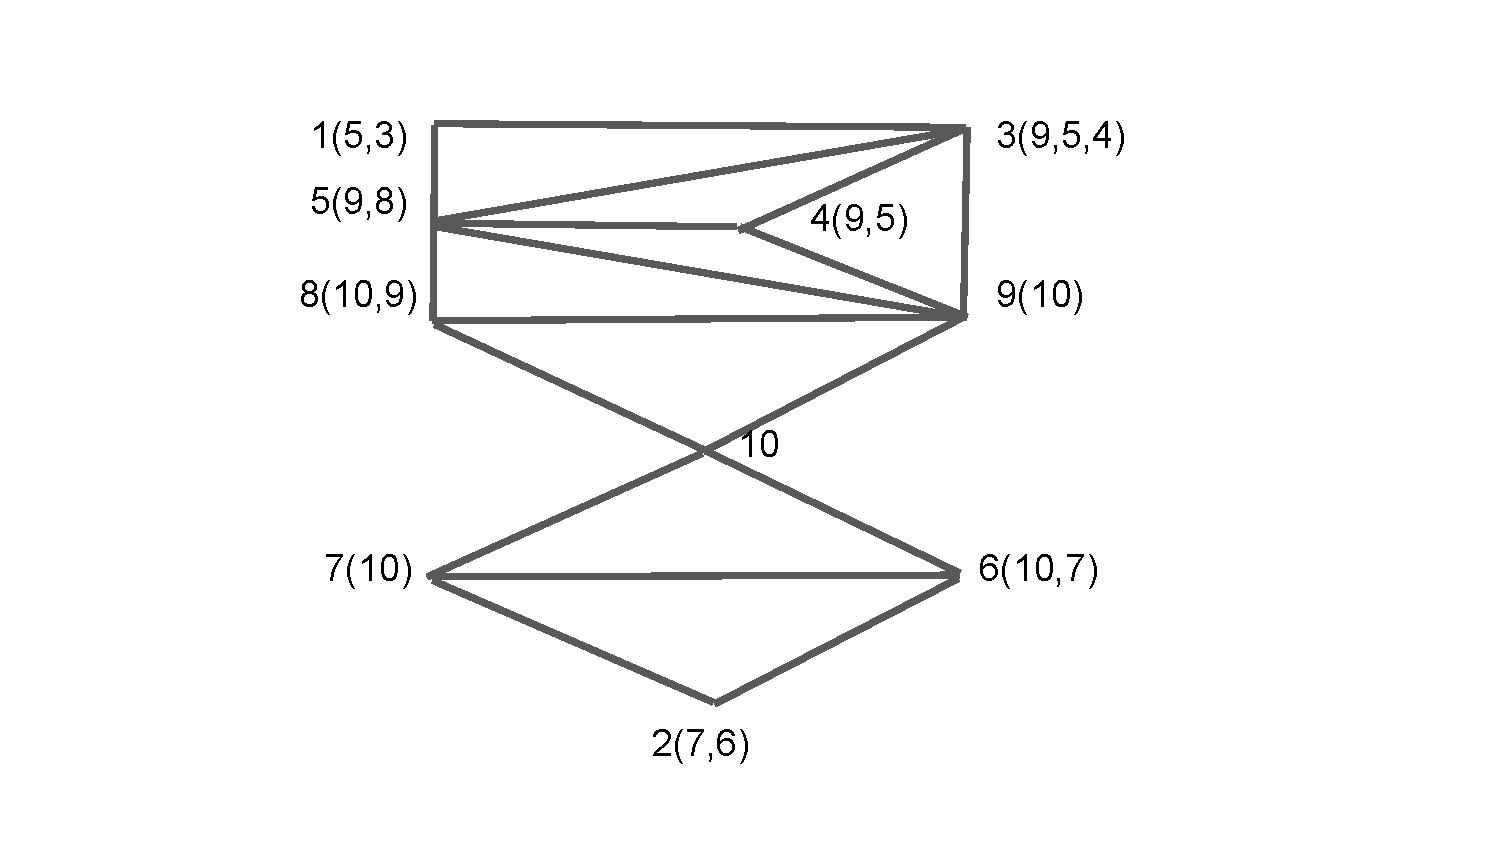
\includegraphics[width=8cm,height=6cm]{figures/lex_illu2}
\caption{Final labels and perfect elimination order generated when apply Lexicographic Breadth First Search}
\label{lex_illu}
\end{figure}

\begin{theorem}
An undirected graph $G = (V,E)$ is chordal if and only if the ordering $\sigma$ produced by Algorithm \ref{lexbfs} is a perfect elimination ordering. 
\end{theorem}

\begin{proof}
If the ordering produced is a perfect elimination ordering, then the graph is apparently chordal by theorem \ref{peo}.

For the other direction of the theorem, suppose $G$ is chordal and in the returned ordering, a vertex $x$ is not simplicial, then we can choose vertices $x_1$ and $x_2$ to be $x$'s neighbors but $x_1 x_2$ is not an edge with largest $x_2$ possible. Since $x x_2$ is an edge and $x_1 x_2$ is a non-edge, $x_2$ is not the vertex that made a difference in $x$ and $x_1$'s label, their label is already distinguished by before processing $x_2$, otherwise, $x$ will be after $x_1$. Suppose $x_3$ being the largest vertex $x x_3 \notin E$ and $x_1 x_3 \in E$, we know that $x x_3$ must be an edge, $x_1 x_3$ must be an non-edge. Moreover, $x_2 x_3$ is required to be a non-edge, if not, it will create a chordless cycle. Similar argument can be derived for $x_4$ in Figure\ref{peo_proof_1}. Clearly, this procedure continues indefinitely, but the graph is finite. Therefore, 
the vertex $x$ must be simplicial and theorem is proved.
\end{proof}

\begin{figure}[H]
\centering
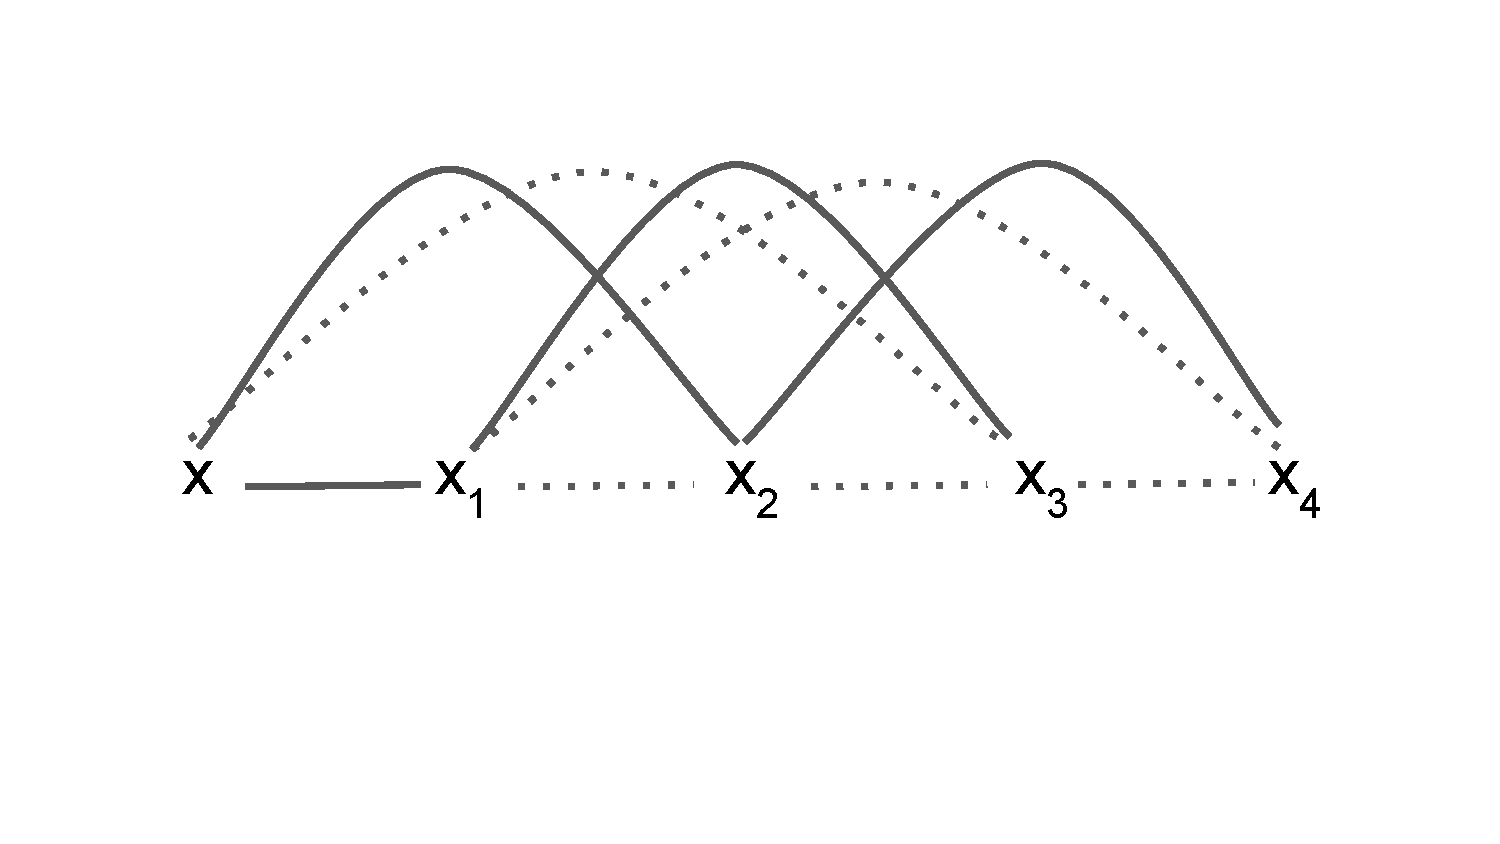
\includegraphics[width=8cm]{figures/lex_proof1}
\caption{Non-simplicial vertex in returned ordering}
\label{peo_proof_1}
\end{figure}

Having proved the correctness of Algorithm \ref{lexbfs}, let us now analyze its complexity. For efficient implementation of Lex-BFS, we do not actually calculate the labels but we keep the numbered vertices in lexicographic order. The idea of maintaining the lexicographic order is to use queue of sets. Vertices in one set are considered to have the same label, but this label is not recorded. 

\begin{algorithm}[H]

\SetAlgoLined
%\TitleOfAlgo{Lexicographic Breadth-First Search Implementation}
%\BlankLine
\caption{Lexicographic Breadth-First Search Implementation}
\label{lexbfs_implementation}
\KwData{ The adjacency sets of an undirected graph $G(V,E)$ }
\KwResult{ An ordering $\sigma$ of the vertices}
\BlankLine
\Begin
{    
	Initialize a sequence $Q$ of sets, to contain a single set containing all vertices;
    
    Initialize the output ordering of vertices to be empty;
    
    \While{$Q$ is not Empty}{
    
    	Find and remove a vertex $v$ from the first set in Q;
        
        If the first set in $Q$ is now empty, remove it from Q;
        
        Add v to the end of the output ordering;
        
		\For{each edge $vw$ such that $w$ still belongs to a set S in Q}
        {
			If the set $S$ containing $w$ has not yet been replaced while processing $v$, create a new empty replacement set $T$ and place it prior to S in the sequence; otherwise, let $T$ be the set prior to $S$;
			
            Move $w$ from $S$ to $T$, and if this causes $S$ to become empty remove $S$ from $Q$;
        }
    }
   
}       
\end{algorithm}

Both the queue and the set is implemented by a doubly linked list, the insertion and deletion of sets in the queue take $O(1)$ time. It is easy to verify that the For loop takes $O(1)$ time for each edge processed. Thus, Algorithm \ref{lexbfs_implementation} runs in $O(|V|+|E|)$ time.

So far, we have a linear time algorithm to produce a prefect elimination ordering if $G=(V,E)$ is a chordal graph. However, this algorithm produces an order no matter whether $G$ is chordal or not. Therefore, a way to test whether this ordering is a correct perfect elimination ordering is needed. This algorithm is Algorithm\ref{peo_test}.

\begin{algorithm}[H]

\SetAlgoLined
%\TitleOfAlgo{Perfect Elimination Ordering Verification}
%\BlankLine
\caption{Perfect Elimination Ordering Verification}
\label{peo_test}
\KwData{ An ordering $\sigma$ of the vertices}
\KwResult{ Boolean }
\BlankLine
\Begin
{    
	\For{all vertices v}{
    $A(v) \leftarrow \emptyset$ }
   \For{$i \leftarrow 1$ to $n-1$}
   {
   		$v \leftarrow \sigma(i)$;
        
        $X \leftarrow \{x \in N(v)|\sigma^{-1}(v) < \sigma^{-1}(x)\}$
        
        \If{$X = \emptyset$}{ go to line 13}
        
        $u \leftarrow \sigma(min \{\sigma^{-1}(x)|x \in X \})$
        
        concatenate $X-\{u\}$ to A(u);
        
        \If{$A(v) - N(v) \neq \emptyset$}{ return "false"}
        
        
        
	}
    return "true"
}       
\end{algorithm}

\begin{theorem}
\cite{rose1976algorithmic}
Algorithm \ref{peo_test} correctly tests whether or not an ordering $\sigma$ of the vertices is a perfect elimination ordering.
\end{theorem}


% \begin{proof}
% TO BE DONE
% The algorithm returns "false" during the $\sigma^{-1}(u)$-th iteration if and only if there exists v,u,w()..NOT FINISHED
% \end{proof}


